

\chapter{\uppercase{Existing Works}}

Several workarounds exist that attempt to alleviate the issue, with one used in practice, but none are fully successful. Other DNS systems already exist, including some that are distributed, but they are either not applicable, or their design makes it extremely challenging to integration into the Tor environment. Two primary problems occur when attempting to use existing DNS systems: being able to prove the correlation of ownership between the DNS name and the hidden service, and the leakage of information that may compromise the anonymity of the hidden service or its operator. As hidden services are only known by their public key and introduction points, it is not easy to use only the hidden service descriptor to prove ownership, and there are privacy and security issues with requiring any more information. Due to these problems, no existing works have been yet integrated into the Tor environment, and the one workaround that is used in practice remains only partially successful.


%DNSNMC + okTurtles = http://diyhpl.us/~bryan/papers2/security/DNSNMC%20okTurtles%20-%20DNSNMC%20replaces%20Certificate%20Authorities%20with%20Namecoin%20and%20fixes%20HTTPS%20security.pdf

%Namecoin as authentication for public-key cryptography = http://www.diva-portal.org/smash/get/diva2:730344/FULLTEXT01.pdf

%Providing better confidentiality and authentication on the Internet using Namecoin and MinimaLT = file:///home/jesse/Downloads/paper.pdf

%Group Spreading: A Protocol for Provably Secure Distributed Name Service = http://www.cs.jhu.edu/~baruch/RESEARCH/Research_areas/Peer-to-Peer/2004_ICALP/icalp04.pdf

%Secure Distributed DNS = http://ieeexplore.ieee.org/stamp/stamp.jsp?tp=&arnumber=1311912

%Domain name resolution using a distributed DNS network = https://www.google.com/patents/US7725602

%P2PNS: A Secure Distributed Name Service for P2PSIP = http://ieeexplore.ieee.org/stamp/stamp.jsp?tp=&arnumber=4517442


\section{Encoding Schemes}

In an attempt to address the readability and the memorability of hidden service domain names, two changes to the encoding of domain names have been proposed, with one used in practice.

Shallot, originally created by an anonymous developer sometime between 2004 and 2010, is an application which uses OpenSSL to generate many RSA hidden service keys in an attempt to find one that has a desirable hash, such as one that begins with a meaningful noun.\cite{KatmagicShallot} By brute-forcing the domain key-space, Shallot will eventually find a domain that is meaningful and partially memorable to the hidden service operator. Shallot was used by Blockchain.info (blockchainbdgpzk.onion), by Facebook (facebookcorewwwi.onion), and by many other hidden services in an attempt to make their domain name appear less random. However, Shallot only partially successful because the size of the domain key-space is too large to be fully brute-forced in any reasonable length of time. For example, on a 1.5 GHz processor, Shallot is expected to take approximately 25 days to find a key whose hash contains 8 custom letters out of the 16 total.\cite{KatmagicShallot} Tor Proposal 224 makes this solution even worse as it suggests 32-byte domain names which embed an entire ECDSA hidden service key in base32.\cite{Proposal224} Although prefixing the domain name with a meaningful word helps identify a hidden service at a glance, it does nothing to alleviate the logistic problems of entering a hidden service domain name, including the remaining random characters, manually into the Tor Browser.

A different encoding scheme was proposed in 2011 by Simon Nicolussi, who suggested that encoding the key hash as a series of words, using a dictionary known in advance by all parties. The list of words would then represent the domain name, rather than base58. While this scheme would improve the memorability of hidden services, the words cannot all be chosen by the hidden service operator, and brute-forcing with Shallot would again only be partially successful due to the large key-space. Therefore this solution could be used to generate some words that relate to the hidden service in a meaningful way, but this scheme is only a partial solution.\cite{NicolussiThesis2011}

These schemes do not change the underlying hidden service protocol, they just attempt to increase the readability of the domain names in Tor Browser. Compared against our original requirements, they meet the anonymity for registration and lookups due to Tor circuits, the confirmability because the domain is the hash of the public key, the uniqueness of domain names due to the collision-free property of SHA-1, the distributed requirement by way of the distributed hashtable stored throughout the Tor network, and resistance to malicious modifications because of the strong association between domain names and the hidden service key. However, it fails to meet the simplicity requirement because although hidden service domain names are entered in the traditional manner into the Tor Browser, the domain names are not entirely human-meaningful nor memorable. The domain names continue to suffer from usability problems, only partially alleviated by these encoding schemes. These workarounds do not introduce any new DNS systems or change the existing Tor hidden service protocol in any way that allows for customized domain names, but these partial solutions are worthy of mention nevertheless.



\section{Clearnet DNS}

The Internet Domain Name Service (DNS) was originally designed in 1983 as a hierarchical naming system to link domain names to Internet Protocol (IP) addresses and translate one to the other. IP addresses specify the location of a computer or device on a network and domain names identify that resource. Domain names therefore operate as an abstraction layer, allowing servers to be moved to a different IP address without loss of functionality. The names consist of a top-level domain (TLD) that is prefixed by a sequence of labels, delimited by dotes. The labels divide the DNS system into zones of responsibility, where each label can be unique within that zone, but not necessarily across different zones. Each label can consist of up to 63 characters and the domain names can be up to 253 characters in total length. In contrast to IP addresses, domain names are human-meaningful and easily memorized, so DNS is a crucial component to the usability of the Internet.

The Clearnet DNS system suffers from several significant shortcomings that make it inappropriate for use by Tor hidden services. First, responses to DNS queries are not authenticated by digital signatures, so spoofing by a MITM attack is possible. Secondly, queries and responses are not encrypted, so it is easy for anyone wiretapping port 53 to correlate end-users to their activities, even if the communication to those websites is protected by TLS/HTTPS. Third, it suffers from DNS cache poisoning, in which an attacker pretends to be an authoritative server and sends incorrect or malicious records to local DNS resolvers. Finally, owning a TLD specifically for Tor hidden services (such as .tor) is prohibitively expensive. While DNS looks traditionally go through the Tor circuit and are resolved by Tor exit nodes, the shortcomings of the Clearnet DNS system make it unsuitable for our purposes.

The traditional Clearnet DNS system meets only a few of our requirements; registrations require a significant of identifiable and geographic information and thus are far from anonymous, lookups occur without encryption or signatures and are therefore neither anonymous nor privacy-enhanced, registrations are by default not publically confirmable but can be made so through use of an expensive SSL certificate from a central authority, the system is zone-based but is managed by centralized organizations and is therefore only partially distributed, and while it is very simple to use, extremely popular, and backwards compatible with TCP/IP, a Tor-specific TLD does not exist and falsifications of registrations is possible in a number of different ways. For its many security issues we therefore dismiss it as a possible solution.



\section{Namecoin}

Namecoin (NMC) is a decentralized peer-to-peer information registration and transfer system, developed by Vincent Durham in early 2011. It was the first fork of Bitcoin and as such inherits most of Bitcoin's design and capabilities. Like Bitcoin, a digital cryptocurrency created by pseudonymous developer Satoshi Nakamoto in 2008, Namecoin holds name records and transactions in a public ledger known as a blockchain. Users may hold Namecoins, and may prove ownership and authorize transactions with their private secp256k1 ECDSA key. Each transaction is a transfer of ownership of a certain amount of NMC from one public key to another, and as all transactions are recorded into the blockchain by the Namecoin network, all Namecoins can be traced backwards to the point of origin. Purchasing a name-value pair, such as a domain name, consumes 0.01 Namecoins, thus adding value and some expense to names in the system. Durham added two rules to Namecoin not present in Bitcoin: names in the blockchain expire after 36,000 blocks (about every 250 days) unless renewed by the owner and no two unexpired names can be identical. Namecoin domain names use the .bit TLD, which is not in use by ICANN.

\begin{figure}[htbp]
	\centering
	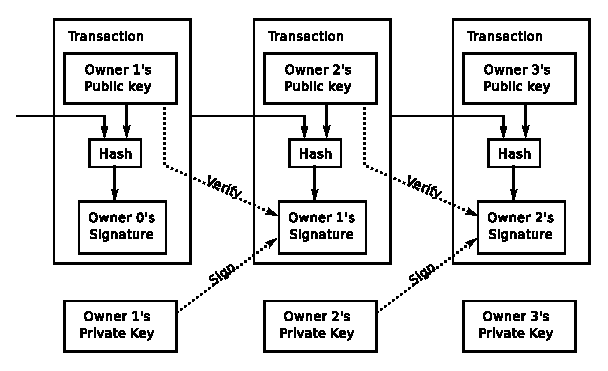
\includegraphics[width=0.6\textwidth]{images/bitcoin_transaction.eps}
	\caption{Three traditional Namecoin transactions.}
	\label{fig:figure7}
\end{figure}

The blockchain data structure is Nakamoto's novel answer to the problem of ensuring agreement of critical data across all involved parties. This prevents the double-spending of Bitcoins, or in Namecoin's case the prevention of duplicate names. Starting from an initial genesis block, all blocks of data link to one another by referencing the hash of a previous block. Blocks are generated and appended to the chain at a relatively fixed rate by a process known as mining. The mining process is the solving of a proof-of-work (PoW) problem in a scheme similar to Adam Back's Hashcash: find a nonce that when passed through two rounds of SHA256 ($ \textrm{SHA}256^{{2}} $) produces a value less than or equal to a target $ T $. This requires a party to perform on average $ \frac{1}{Pr[H \leq T]} = \frac{2 ^ {{256}}}{T} $ amount of computations, but it is easy to verify afterwards that $ \textrm{SHA}256^{{2}}(\textrm{msg} || n) \leq T $. Once the PoW is complete, the block (containing the back-reference hash, a list of transactions, and the PoW variables) is broadcasting to rest of the network, thus forming an append-only chain whose validity everyone can confirm. As each block is generated, the miner receives fresh Namecoins, thus introducing newly-minted Namecoins into the system at a fixed rate. Blocks cannot be modified retrospectively without requiring regeneration of the PoW of that block and all subsequent blocks, so the PoW locks blocks in the chain together. Nodes in the Namecoin network collectively agree to use the blockchain with the highest accumulation of computational effort, so an adversary seeking to modify the structure would need to recompute the proof-of-work for all previous blocks as well as out-perform the network, which is currently considered infeasible.\cite{Okupski2014}

\begin{figure}[htbp]
	\centering
	
\includegraphics[width=0.6\textwidth]{images/Blockchain-2.eps}
	\caption{A sample blockchain.}
	\label{fig:figure6}
\end{figure}

Each block in the blockchain consists of a header and a payload. The header contains a hash of the previous block's header, the root hash of the Merkle tree built from the transactions in this block, a timestamp, a target $ T $, and a nonce. The block payload consists of a list of transactions. The root node of the Merkle tree ensures the integrity of the transaction vector: verifying that a given transaction is contained in the tree takes $ log(n) $ hashes, and a Merkle tree can be built $ n * log(n) $ time, ensuring that all transactions are accounted for. The hash of the previous block in the header ensures that blocks are ordered chronologically, and the Merkle root hash ensures that the transactions contained in each block are order chronologically as well. The target $ T $ changes every 2016 blocks in response to the speed at which the proof-of-work is solved such that Bitcoin miners take two weeks to generate 2016 blocks, or one block every 10 minutes. The change in target ensures that the difficulty of the proof-of-work remains relatively constant as processing capabilities increase according to Moore's Law. In the event that multiple nodes solve the proof-of-work and generate a new block simultaneously, the forked block becomes orphaned, the transactions recycled, and the network converges to follow the blockchain with the longest path from the genesis node, thus the one with the most amount of PoW behind it.\cite{Okupski2014}

Namecoin is particularly noteworthy in that it was the first systems to prove Zooko's Triangle false in a practical sense. The blockchain public ledger is held by every node in the distributed network, and human-meaningful names can be owned and placed inside it. The rules of the Namecoin network tell all participants to ensure that there are no name duplicates, and anyone holding the blockchain can verify this property. Names cannot be inserted retroactively due to the PoW, so these properties are ensured. Thus, Namecoin achieves all three properties in Zooko's Triangle. Namecoin is the most commonly-used alternative DNS system and is noted for its security and censorship resistance. In 2014, Namecoin was recognized by ICANN as the most well-known example of a PKI and DNS system with an emphasis of distributed control and privacy, a growing trend in light of the revelations about the US National Security Agency (NSA) by Edward Snowden.\cite{NamecoinReportICANN} %https://www.icann.org/en/system/files/files/report-21feb14-en.pdf

%https://bitinfocharts.com/
While Namecoin is perhaps the most well-known secure distributed DNS system, it too is not applicable to Tor's environment. One of the main problems is one of practicality: it is unreasonable to require all Tor users to be able to download the entire Namecoin blockchain, which currently stands at 2.05 GB as of January 2015,\cite{BitInfoCharts} in order to know DNS records and verify the uniqueness of names. While this burden could be shifted to Tor nodes, Tor clients must then be able to trust the nodes to return an accurate record or even the correct block that contained that record. If the client queried the Namecoin network for DNS information through a Tor circuit, they would have no way of verifying the accuracy of the information without holding a complete blockchain to verify it. Secondly, the hidden service operator would have to prove that he owned both the ECDSA private key attached to the Namecoin record and the private RSA key attached to his hidden service in a manner that is both publicaly confirmable and didn't compromise his identity or location. These problems make Namecoin difficult to integrate securely into Tor. While we recognize Namecoin for its novelty and EsgalDNS shares some similarities with Namecoin, Namecoin itself is not a viable solution here.

Namecoin meets only some of our initial requirements; anonymity during registration can be met when the hidden service operator uses a Tor circuit, anonymity or privacy-enhancement during lookup can be met when the Tor client uses a Tor circuit for the query, public confirmability of the name to the hidden service is not easily met, domain name uniqueness is met by the Namecoin network but not easily proven without access to the entire blockchain, the distributed property is met by the nature of the network, simplicity is not fully met by Namecoin and further software would have be developed to accomplish this objective for Tor integration, backwards compatibility is unknown but could theoretically be met by certain designs, and resistance to malicious modifications or falsifications is met by the network but again not easily proven without access to the entire blockchain.
